% interactcadsample.tex
% v1.03 - April 2017

\documentclass[]{interact}

\usepackage{epstopdf}% To incorporate .eps illustrations using PDFLaTeX, etc.
\usepackage{subfigure}% Support for small, `sub' figures and tables
%\usepackage[nolists,tablesfirst]{endfloat}% To `separate' figures and tables from text if required

\usepackage{natbib}% Citation support using natbib.sty
\bibpunct[, ]{(}{)}{;}{a}{}{,}% Citation support using natbib.sty
\renewcommand\bibfont{\fontsize{10}{12}\selectfont}% Bibliography support using natbib.sty

\theoremstyle{plain}% Theorem-like structures provided by amsthm.sty
\newtheorem{theorem}{Theorem}[section]
\newtheorem{lemma}[theorem]{Lemma}
\newtheorem{corollary}[theorem]{Corollary}
\newtheorem{proposition}[theorem]{Proposition}

\theoremstyle{definition}
\newtheorem{definition}[theorem]{Definition}
\newtheorem{example}[theorem]{Example}

\theoremstyle{remark}
\newtheorem{remark}{Remark}
\newtheorem{notation}{Notation}


% tightlist command for lists without linebreak
\providecommand{\tightlist}{%
  \setlength{\itemsep}{0pt}\setlength{\parskip}{0pt}}



\usepackage{lscape}
\usepackage{hyperref}
\usepackage[utf8]{inputenc}
\def\tightlist{}
\usepackage{setspace}
\doublespacing


\begin{document}


\articletype{ARTICLE TEMPLATE}

\title{Automated reading of residual plots with computer vision models}


\author{\name{Weihao Li$^{a}$}
\affil{$^{a}$Department of Econometrics and Business Statistics, Monash
University, Clayton, VIC, Australia}
}

\thanks{CONTACT Weihao
Li. Email: \href{mailto:weihao.li@monash.edu}{\nolinkurl{weihao.li@monash.edu}}}

\maketitle

\begin{abstract}
TBD.
\end{abstract}

\begin{keywords}
TBD
\end{keywords}

\hypertarget{introduction}{%
\section{Introduction}\label{introduction}}

Residuals, within regression analysis, represent the differences between
fitted values and observed data points, capturing the unexplained
elements in the regression model. The practice of plotting residuals,
advocated by influential regression literature
\citep{cook1982residuals, draper1998applied, belsley1980regression, montgomery1982introduction},
serves as a standard procedure in regression diagnostics. This visual
examination is crucial for identifying deviations from the model
assumptions like linearity, homoscedasticity, and normality.

Generating a residual plot in most statistical software is often as
straightforward as executing a line of code or clicking a button.
However, accurately interpreting a residual plot can be challenging.
Consider Figure \ref{fig:false-finding} as an example, the residuals
display a triangular shape pointing to the left. While this might
suggest heteroskedasticity, it's important to avoid over-interpreting
the visual pattern. In this case, the fitted model is correctly
specified, and the triangular shape is actually a result of the skewed
distribution of the predictors, rather than indicating a flaw in the
model.

A residual plot can exhibit various visual features, but it's crucial to
recognize that some may arise from the characteristics of predictors and
the inherent randomness of the error, rather than indicating a violation
of model assumptions \citep{li2023plot}. The concept of visual
inference, as proposed by \citet{buja2009statistical}, provides an
inferential framework to assess whether residual plots indeed contain
visual patterns inconsistent with the model assumptions. The fundamental
idea involves testing whether the actual residual plot significantly
differs visually from null plots, which are created using residuals
generated from the null distribution. Typically, this is accomplished
through the lineup protocol. In this approach, the real residual plot is
embedded within a lineup alongside several null plots. If the real
residual plot can be distinguished from the lineup, it provides evidence
for rejecting the null hypothesis.

The practice of delivering a residual plot as a lineup is generally
regarded as a valuable approach. Beyond its application in residual
diagnostics, the lineup protocol has integrated into the analysis of
diverse subjects. For instance,
\cite{loy2013diagnostic, loy2014hlmdiag, loy2015you} illustrate its
applicability in diagnosing hierarchical linear models. Additionally,
\citet{widen2016graphical} demonstrates its utility in geographical
research, while \citet{krishnan2021hierarchical} explores its
effectiveness in forensic examinations.

However, as pointed out by \citet{li2023plot}, a primary limitation of
the lineup protocol lies in its reliance on human judgments. Unlike
conventional statistical tests that can be performed numerically and
automatically in statistical software, the lineup protocol requires
human evaluation of images. This characteristic makes it less suitable
for large-scale applications, given the associated high labour costs and
time requirements.

There is a compelling need to develop an approach that alleviates
people's workload by automating repetitive tasks and providing
standardized results in a controlled environment. The large-scale
evaluation of lineups is impractical without the use of technology and
machines.

The utilization of computers to interpret data plots has a rich history,
with early efforts such as ``Scagnostics'' by \citet{tukey1985computer},
focusing on scatterplot diagnostics. \citet{wilkinson2005graph} expanded
on this work in 2005, introducing graph theoretic scagnostics, which
encompassed nine computable measures applied to planar proximity graphs.
These measures, including ``Outlying,'' ``Skinny,'' ``Stringy,''
``Straight,'' ``Monotonic,'' ``Skewed,'' ``Clumpy,'' and ``Striated,''
aimed to characterize outliers, shape, density, trend, and coherence of
the data.

While this approach has been inspiring, there is a recognition that it
may not capture all the necessary visual features distinguishing actual
residual plots from null plots. An alternative, more promising approach
involves allowing computers to learn the visual feature extraction
function. In essence, this means enabling computers to discern which
visual features are significant for residual diagnostics and how to
extract them. Modern computer vision models, a subset of artificial
intelligence, present a compelling solution to this challenge.

Modern computer vision models often rely on deep neural networks with
convolutional layers \citep{fukushima1982neocognitron}. These layers
leverage hierarchical patterns in data, downsizing and transforming
images by summarizing information in a small space. Numerous studies
have demonstrated the efficacy of convolutional layers in addressing
various vision tasks, including image recognition \citep{rawat2017deep}.

Despite the widespread use of computer vision models in fields like
computer-aided diagnosis \citep{lee2015image}, pedestrian detection
\citep{brunetti2018computer}, and facial recognition
\citep{emami2012facial}, their application in reading data plots remains
limited. While some studies have explored the use of computer vision
models for tasks such as reading recurrence plots for time series
regression \citep{ojeda2020multivariate}, time series classification
\citep{chu2019automatic, hailesilassie2019financial, hatami2018classification, zhang2020encoding},
anomaly detection \citep{chen2020convolutional}, and pairwise causality
analysis \citep{singh2017deep}, the application of reading residual
plots with computer vision models represents a relatively new field of
study.

In this paper, we develop computer vision models and integrate them into
the residual plots diagnostics workflow, filling the gap of\ldots. The
paper is structured as follows: \ldots{}

\begin{figure}

{\centering 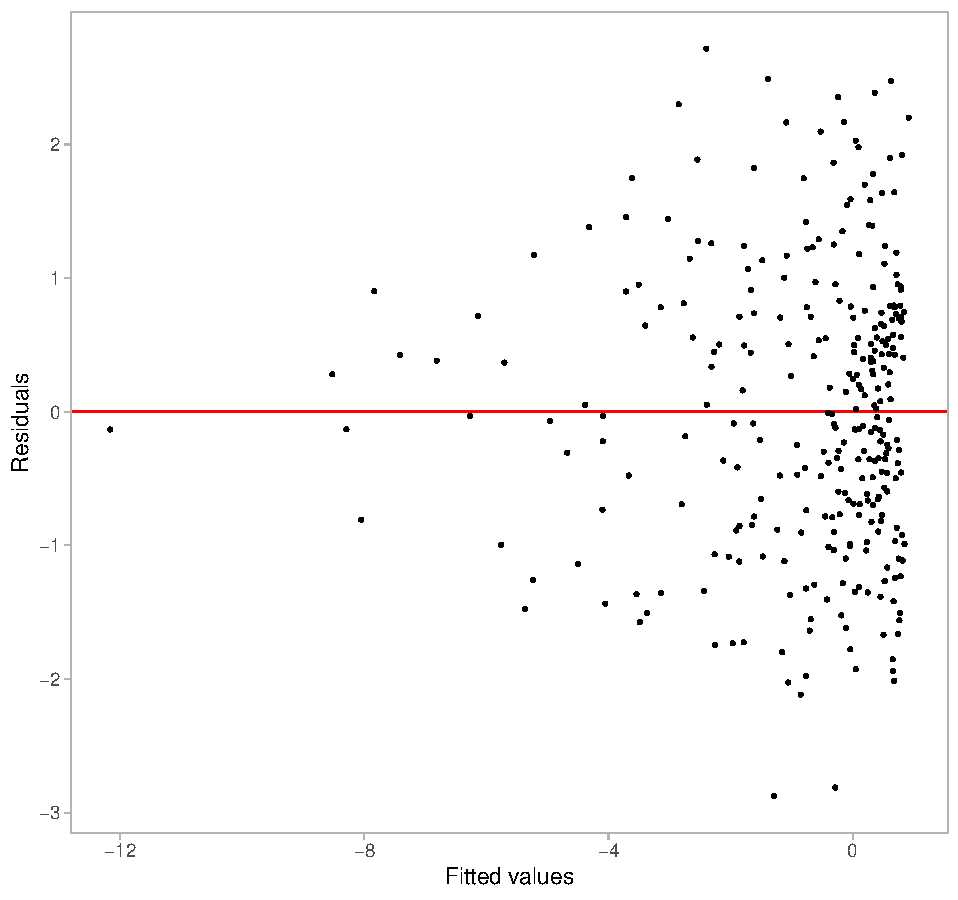
\includegraphics[width=1\linewidth]{paper_files/figure-latex/false-finding-1} 

}

\caption{An example residual vs fitted values plot (red line indicates 0). The vertical spread of the data points varies with the fitted values. This often indicates the existence of heteroskedasticity.}\label{fig:false-finding}
\end{figure}

\hypertarget{methodogology}{%
\section{Methodogology}\label{methodogology}}

\hypertarget{generation-of-simulated-training-data}{%
\subsection{Generation of simulated training
data}\label{generation-of-simulated-training-data}}

\hypertarget{architecture-of-the-computer-vision-model}{%
\subsection{Architecture of the computer vision
model}\label{architecture-of-the-computer-vision-model}}

\hypertarget{training-process-and-hyperparameter-tuning}{%
\subsection{Training process and hyperparameter
tuning}\label{training-process-and-hyperparameter-tuning}}

\hypertarget{results}{%
\section{Results}\label{results}}

\hypertarget{model-evaluation}{%
\subsection{Model evaluation}\label{model-evaluation}}

\begin{itemize}
\tightlist
\item
  Metrics for model performance
\item
  Shap values
\item
  Heatmap
\end{itemize}

\hypertarget{comparison-with-human-visual-inference}{%
\subsection{Comparison with human visual
inference}\label{comparison-with-human-visual-inference}}

\hypertarget{overview-of-the-human-subject-experiment}{%
\subsubsection{Overview of the human subject
experiment}\label{overview-of-the-human-subject-experiment}}

\hypertarget{comparison}{%
\subsubsection{Comparison}\label{comparison}}

\begin{itemize}
\tightlist
\item
  power comparison
\item
  decisions
\end{itemize}

\hypertarget{case-study-1}{%
\subsection{Case study 1: \ldots{}}\label{case-study-1}}

\hypertarget{case-study-2}{%
\subsection{Case study 2: \ldots{}}\label{case-study-2}}

\hypertarget{case-study-3-datasaurus}{%
\subsection{Case study 3: datasaurus}\label{case-study-3-datasaurus}}

\hypertarget{dicussion}{%
\section{Dicussion}\label{dicussion}}

\hypertarget{conclusion}{%
\section{Conclusion}\label{conclusion}}

\begin{itemize}
\tightlist
\item
  Summary of findings
\item
  Contributions to the field
\item
  Future directions for research
\end{itemize}

\bibliographystyle{tfcad}
\bibliography{ref.bib}





\end{document}
